\chapter{Modelling}

We used various techniques for the mass modelling of $\omega$ Centauri, so that we could make a good approximation to its dynamic and stellar mass. In order to do this, we decided to use two components (the stellar and dark matter mass) both following the functional form of the Hernquist profile. In this chapter we present the results of such modelling and discuss their characteristics.    

\section{Hernquist Model}

Our modelling is based on the Hernquist profile (Hernquist 1989).  We use this model because it is a well known model that closely approximates the de Vaucouleurs law for elliptical galaxies and has analytical solutions that can be useful for our computational purposes. As introduced in chapter 2, the density profile for this model is

\begin{equation}
\rho(r)=\frac{M}{2\pi}\frac{a}{r}\frac{1}{\left(r+a\right)^{3}}
\end{equation}

Where $a$ and $M$ are the scalength and total mass associated to the profile that, as we will show, can be associated to the dark or baryonic matter. The profile's cumulative mass is

\begin{equation}
M(r)=M\frac{r^{2}}{(r+a)^{2}}
\end{equation}
 
And the surface brightness 
 
 \begin{equation}
 I(R)=\frac{M}{2\pi a^{2}\Gamma\left(1-s^{2}\right)^{2}}\left[\left(2+s^{2}\right)X(s)-3\right]
 \end{equation}
 
where $s=R/a$, $R$ is the projected radius and:

\begin{equation}
X(s)=\frac{1}{\sqrt{1-s^{2}}}\text{sech}^{-1}s \qquad \rm{for} \qquad 0\leq s\leq1
\end{equation}

\begin{equation}
X(s)=\frac{1}{\sqrt{s^{2}-1}}\sec^{-1}s\qquad \rm{for} \qquad1\leq s<\infty
\end{equation}

For computational simplicity we have written some of the trigonometric functions just like Hernquist did: $\sec^{-1}s = \cos^{-1}(1/s)$ and $\text{sech}^{-1} = \ln[(1+\sqrt{1-s^{2}})/s]$. As mentioned in chapter 2, the line of sight velocity dispersion in the more general case with the anisotropy parameter $\beta$ is given by

\begin{equation}
I(R)\sigma_{p}^{2}(R)=\frac{2}{\Gamma}\int_{R}^{\infty}\left(1-\beta\frac{R^{2}}{r^{2}}\right)\frac{\rho\bar{v_{r}^{2}}rdr}{\sqrt{r^{2}-R^{2}}}
\end{equation}

Where $\Gamma$ is the mass-to-light ratio. The radial velocity dispersion (introduced in chapter 2), in terms of the potential and the density is

\begin{equation}
\bar{v_{r}^{2}}=\sigma_{r}^{2}=\frac{1}{\rho(r)}\int_{r}^{\infty}\rho(r)\frac{d\phi}{dr}dr
\end{equation}

Where 

\begin{equation}
\frac{d\phi}{dr}=\frac{GM(r)}{r^{2}}
\end{equation}

So the projected velocity dispersion becomes:

\begin{equation}
\sigma_{p}^{2}(R)=\frac{2G}{I(R)\Gamma}\int_{R}^{\infty}\left(1-\beta\frac{R^{2}}{r^{2}}\right)\left(\int_{r}^{\infty}\frac{\rho(r)M(r)}{r^{2}}dr\right)\frac{rdr}{\sqrt{r^{2}-R^{2}}}
\end{equation}

We do various experiments for our modelling, the simplest of all models is the one where we assume that the cluster has just one mass component, in this case there only will be one mass contribution (stellar mass) and only one scalength (the stellar scalength) so the solution of the last equation would be:

\begin{equation}
\sigma_{p}^{2}(R)=\frac{GM^{2}a}{I(R)\Gamma\pi}\int_{R}^{\infty}\alpha(r)\left(\frac{\log{\left(\frac{a+r}{r}\right)}}{a^{5}}-\frac{25a^{3}+52a^{2}r+42ar^{2}+12r^{3}}{12a^{4}\left(a+r\right)^{4}}\right)dr
\end{equation}

Where $a$ is the scalength and where, in order to shorten the equation we take $\alpha(r)$ as 

\begin{equation}
\alpha(r)=\left(1-\beta\frac{R^{2}}{r^{2}}\right)\frac{r}{\sqrt{r^{2}-R^{2}}}
\end{equation}

Now, as we want to focus on the dark matter content of the cluster, we assume that the mass of the cluster is the sum of the mass of stars and the mass of non-baryonic matter so that their contributions to the density and mass profiles become:

\begin{equation}
\rho(r)=\rho_{s}(r)+\rho_{dm}(r)\qquad and \qquad M(r)=M_{s}(r)+M_{dm}(r)
\end{equation} 

In this case, the projected velocity dispersion takes a much more complicated form as follows:

\begin{equation}
\begin{aligned}	
\sigma_{p}^{2}(R) &= \frac{G}{I(R)\Gamma\pi}\int_{R}^{\infty}\alpha(r)\Biggl[\underbrace{\int_{r}^{\infty}\frac{M_{s}^{2}a_{s}dr}{r\left(r+a_{s}\right)^{5}}}_{\mathbf{A}(r)}+\underbrace{\int_{r}^{\infty}\frac{M_{s}M_{dm}a_{s}dr}{r\left(r+a_{s}\right)^{3}\left(r+a_{dm}\right)^{2}}}_{\mathbf{B}(r)}\right\\     &+ \underbrace{\int_{r}^{\infty}\frac{M_{dm}M_{s}a_{dm}dr}{r\left(r+a_{dm}\right)^{3}\left(r+a_{s}\right)^{2}}}_{\mathbf{C}(r)}+\underbrace{\int_{r}^{\infty}\frac{M_{dm}^{2}a_{dm}dr}{r\left(r+a_{dm}\right)^{5}}}_{\mathbf{D}(r)}\Biggr] dr
\end{aligned}
\end{equation}

The functional form of the density involves the use of a stellar scalength ($a_{s}$), a dark matter scalength ($a_{dm}$), a stellar mass ($M_{s}$) and a dark matter mass ($M_{dm}$). Now, the integrals $\mathbf{A}(r),\mathbf{B}(r),\mathbf{C}(r)$ and $\mathbf{D}(r)$ have the following analytical solutions:

\begin{equation}
\textbf{A}(r)=a_{s}\left(-\frac{25a_{s}^{3}+52a_{s}^{2}r+42a_{s}r^{2}+12r^{3}}{12a_{s}^{4}\left(a_{s}+r\right)^{4}}+\frac{\log{\left[\frac{a_{s}+r}{r}\right]}}{a_{s}^{5}}\right)
\end{equation}

\begin{equation}
\textbf{D}(r)=a_{dm}\left(-\frac{25a_{dm}^{3}+52a_{dm}^{2}r+42a_{dm}r^{2}+12r^{3}}{12a_{dm}^{4}\left(a_{dm}+r\right)^{4}}+\frac{\log{\left[\frac{a_{dm}+r}{r}\right]}}{a_{dm}^{5}}\right)
\end{equation}

The crossed terms are

\begin{equation}
\textbf{B}(r)=\frac{\left(M_{s}M_{dm}\right)\left(\mathbf{b_{2}}+\mathbf{b_{3}}+a_{s}\left(-\left(a_{s}-a_{dm}\right)a_{dm}\mathbf{b_{4}}+\mathbf{b_{5}}\right)\right)}{\mathbf{b_{1}}}
\end{equation}

\begin{equation}
With \left\lbrace
\begin{array}{lllll}
\mathbf{b_{1}}=2a_{s}^{2}(a_{s}-a_{dm})^{4}a_{dm}^{2}(a_{s}+r)^{2}(a_{dm}+r)\\
\mathbf{b_{2}}=-2\left(a_{s}-a_{dm}\right)^{4}\left(a_{s}+r\right)^{2}\left(a_{dm}+r\right)\log{r}\\
\mathbf{b_{3}}=2a_{dm}^{2}\left(6a_{s}^{2}-4a_{s}a_{dm}+a_{dm}^{2}\right)
\left(a_{s}+r\right)^{2}\left(a_{dm}+r\right)\log{[a_{s}+r]}\\
\begin{aligned}	
\mathbf{b_{4}} &= 2a_{s}^{4}+4a_{s}^{3}r-2a_{dm}r(a_{dm}+r)+3a_{s}a_{dm}\left(-a_{dm}^{2}+a_{dm}r+2r^{2}\right)\\      &+a_{s}^{2}\left(7a_{dm}^{2}+7a_{dm}r+2r^{2}\right)
\end{aligned}\\
\mathbf{b_{5}}=2a_{s}^{2}\left(a_{s}-4a_{dm}\right)\left(a_{s}+r\right)^{2}\left(a_{dm}+r\right)\log{[a_{dm}+r]}
\end{array}
\right.
\end{equation} 

And

\begin{equation}
\textbf{C}(r)=\frac{\left(M_{dm}M_{s}\right)\left(\mathbf{c_{2}}+\mathbf{c_{3}}+a_{dm}\left(-\left(a_{dm}-a_{s}\right)a_{s}\mathbf{c_{4}}+\mathbf{c_{5}}\right)\right)}{\mathbf{c_{1}}}
\end{equation}

\begin{equation}
With \left\lbrace
\begin{array}{lllll}
\mathbf{c_{1}}=2a_{dm}^{2}(a_{dm}-a_{s})^{4}a_{s}^{2}(a_{dm}+r)^{2}(a_{s}+r)\\
\mathbf{c_{2}}=-2\left(a_{dm}-a_{s}\right)^{4}\left(a_{dm}+r\right)^{2}\left(a_{s}+r\right)\log{r}\\
\mathbf{c_{3}}=2a_{s}^{2}\left(6a_{dm}^{2}-4a_{dm}a_{s}+a_{s}^{2}\right)\left(a_{dm}+r\right)^{2}
\left(a_{s}+r\right)\log{[a_{dm}+r]}\\
\begin{aligned}	
\mathbf{c_{4}} &= 2a_{dm}^{4}+4a_{dm}^{3}r-2a_{s}r(a_{s}+r)+3a_{dm}a_{s}\left(-a_{s}^{2}+a_{s}r+2r^{2}\right)\\      &+a_{dm}^{2}\left(7a_{s}^{2}+7a_{s}r+2r^{2}\right)
\end{aligned}\\
\mathbf{c_{5}} =2a_{dm}^{2}\left(a_{dm}-4a_{s}\right)\left(a_{dm}+r\right)^{2}\left(a_{s}+r\right)\log{[a_{s}+r]}
\end{array}
\right.
\end{equation} 

As we mentioned in chapter 3, we used many databases for projected radial velocities in order to properly do our fit and modelling. The radial velocities as a function of the projected radius are shown in figure 4.1. Because we needed to calculate the projected velocity dispersion profile $\sigma_{p}(R)$, we decided to cut in radial bins as shown in the same figure.

\begin{figure}[]
\centering
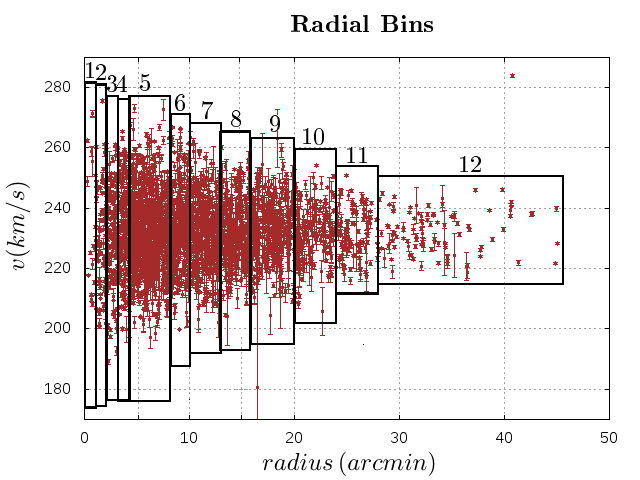
\includegraphics[width=13cm]{images/vel_vs_rad_bins.png}
\caption[Radial bins used to calculate velocity dispersions]{Radial velocities vs projected radius in arcmin. The data is taken from all the databases that gave us a good level of confidence, note that all the data have their respective error. The figure also shows the adial bins that we used to calculate the radial projected velocity dispersion in the cluster using equation 4.20}
\end{figure}

The velocity dispersion is estimated as the standard deviation of the velocity in each radial bin because we want to see how much the velocity data deviates from the median, and it is calculated with the formula

\begin{equation}
\sigma = \sqrt{\frac{\sum_{i=1}^{n}\left(v_{i}-v\right)^{2}}{N}}
\end{equation}

Where $v$ is the median of the velocities in each bin. To see if the estimation is well made, we plot histograms for each bin to see if the velocities follow a Gaussian behaviour, and where the number of bars in each histogram is given by the square root of the number of velocities in each bin. For some of the radial bins of our profile, the histograms are shown in figure 4.2 where we see that the velocities follow a nearly Gaussian distribution per bin, which justifies the use of equation 4.20.

\begin{figure}[]
\centering
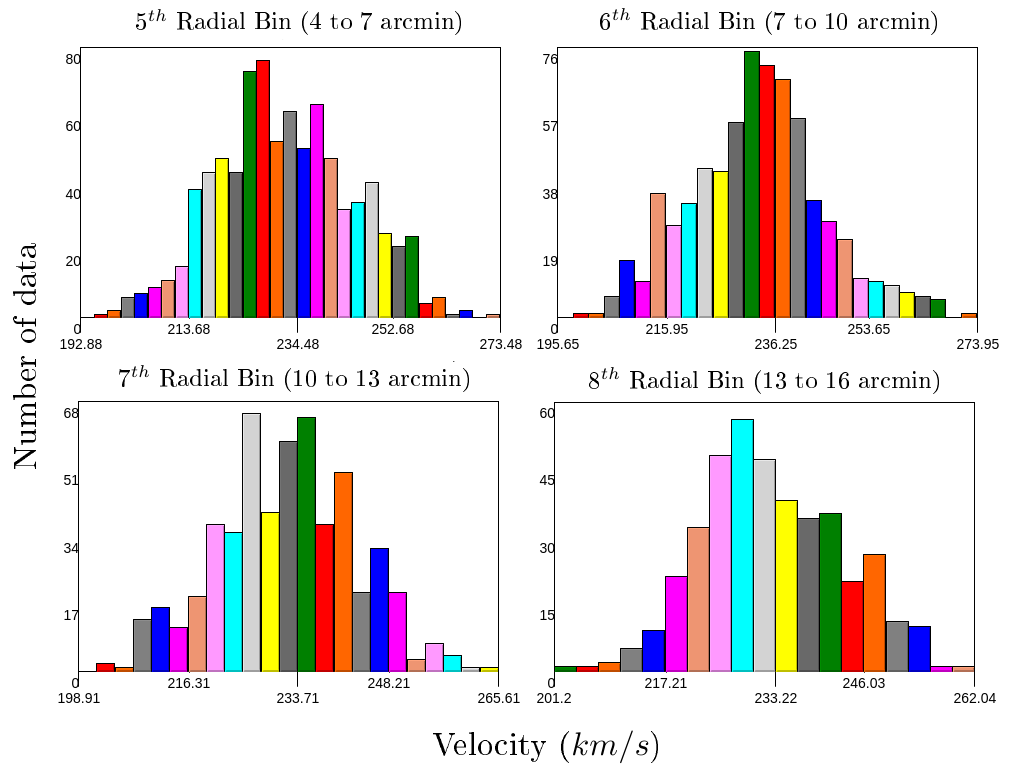
\includegraphics[width=15cm]{images/bines.png}
\caption[Histograms for some of the radial bins in our profile]{The histograms for the $5^{th}$, $6^{th}$, $7^{th}$ and $8^{th}$ radial bins. Note that the frequency of repetition of the velocities displayed in bars follows a Gaussian behaviour which suggests that the method used to calculate the velocity dispersion in accurate enough for the modelling.}
\end{figure}

In order to do a proper modelling and fitting we need to take into account the error associated with $\sigma_{p}$. Because all the databases provided the associated error to the measurements of the radial velocities, we made the proper calculation of the error of the velocity dispersion using the general error propagation formula

\begin{equation}
\sigma(v\pm\Delta v)\approx \sigma(v)\pm \underbrace{\frac{\partial \sigma}{\partial v}\Delta v}_{\Delta \sigma}
\end{equation}

So the error of the projected velocity dispersion is estimated as

\begin{equation}
\Delta \sigma = \frac{1}{\sqrt{N}}\left(\sum_{i=1}^{n}\left(v_{i}-v\right)^{2}\right)^{-1/2}\sum_{i=1}^{n}\left(v_{i}-v\right)\Delta v
\end{equation}

With the radial projected velocity dispersion (and its error) we can start with the fitting to find the optimized parameters in our various experiments taking into account several physical constraints. 

\section{Setting constraints}

\subsection{Stellar mass}

The stellar mass content of Globular Clusters and Galaxies can be studied through the determination of the stellar populations inside those systems because we have clear knowledge about how their photometric properties relate to their mass. If we have information about the relative abundance of the stellar populations inside the stellar system, then we can infer the total mass of the cluster by summing up all of these contributions. 

The determination of the stellar populations can be done using STARLIGHT, which is a Fortran-based program that fits an observed integrated spectrum (the central region of Omega Centauri in our case) with a model spectrum which is the sum of $N_{*}$ spectral components from a pre-defined and pre-processed set of base spectra. The program does as many iterations as the user decides to sum up the different template spectra until a good fitting of the spectral lines has been made to the observed spectrum. 

The output of the program after the execution contains the created spectrum (wavelength and intensity) and the approximate percentage of each of the stellar populations inside the stellar system that we use for the determination of the total mass of the cluster.

First, one must prepare the observed spectrum before running STARLIGHT, the spectrum has to be wavelength and flux calibrated, taking into account the bad-pixel removal. Very importantly in the context of mass analysis, the spectrum has to be extinction corrected so that the units of flux relate properly to the units of the templates in STARLIGHT.     

The extinction correction for our observed spectrum is given by

\begin{equation}
f_{obs}(\lambda)=f_{int}(\lambda)10^{-0.4A_{\lambda}}
\end{equation}

Where $A_{\lambda}=0.213$ in the I filter around $8000 \textrm{\AA}$, around the wavelength range of our spectrum. 

In our case, we have to multiply by a factor of $1.216746$ the intensity of the spectrum to correct of extinction. After we apply the extinction correction to the spectrum and create an ASCII table with the wavelength, intensity and error columns, we have an spectrum that is ready to be processed with STARLIGHT. We can see both spectra (the one that has been extinction corrected and the one that has not) in figure 4.3 and note the significant shift in the flux for the corrected spectrum.

\begin{figure}[H]
\centering
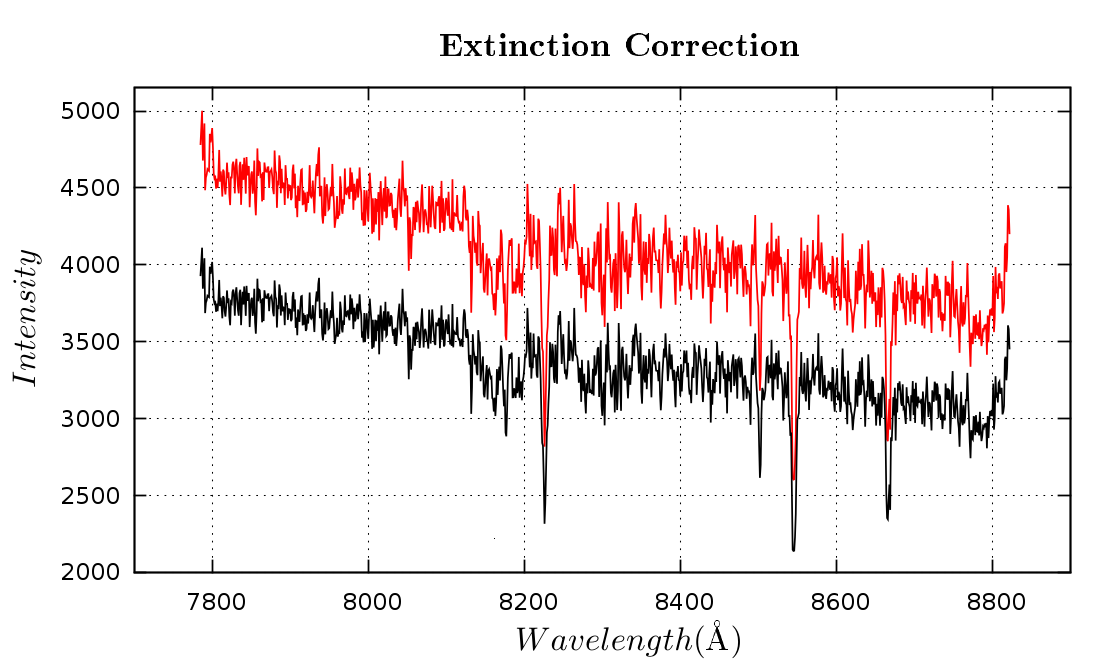
\includegraphics[width=10cm]{images/extinction.png}
\caption[Extinction Correction]{This figure shows an integrated spectrum of the central region of Omega Centauri before and after the extinction correction is applied. The black line has the original flux values and the black line has the corrected flux, that is, the flux that would be observed if there wasn't any interstellar medium that obscures the light coming from the object.}
\end{figure}

Before running STARLIGHT one must assure that the wavelength range is correctly specified in the configuration file that also includes the database of the template spectra and the bad data organized in a mask file. When all of these are ready it is straightforward to run STARLIGHT with the following command (in a linux-based computer):

\begin{center}
./StarlightChains\_v04.exe $<$ Omega\_cen.in
\end{center}

The synthetic spectrum and the original one are shown in figure 4.4 where we can see that the created synthetic spectrum keeps the prominent lines, the small features of the original spectrum, the form and the scale of the absorption lines and it models our spectrum so well that the two spectra had to be y-shifted in the figure to visualize the small differences.

\begin{figure}[]
\centering
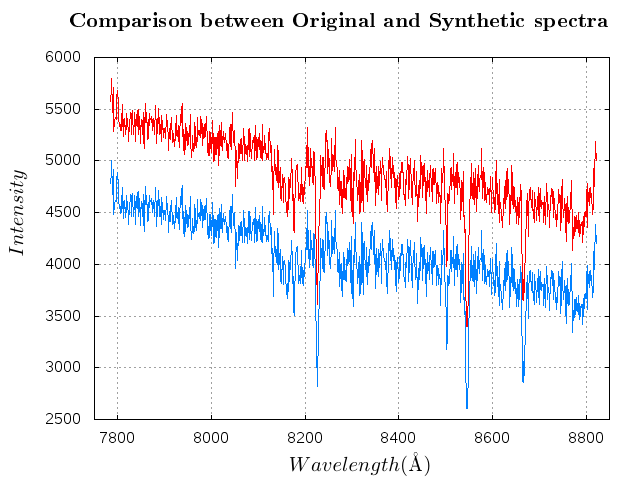
\includegraphics[width=10cm]{images/comparison.png}
\caption[Synthetic spectrum of STARLIGHT]{Synthetic spectrum of Starlight in red, shifted in the y axis for doing the comparison with the original spectrum of Omega Centauri in blue. Note how similar the spectra are, meaining that the results given by Starlight were very accurate}
\end{figure}
 
Now, besides the synthetic spectrum, the output file contains some useful results that one can use to estimate the mass of the stellar system. In our case, the relevant parameter that STARLIGHT gives is the ``stellar mass parameter":

\begin{equation}
M_{cor\_tot} = 3.29446 \times 10^{7} M_{\odot}/cm^{2}
\end{equation}

And using the formula for the total mass in units of solar masses:

\begin{equation}
M_{s}(M_{\odot})=M_{cor\_tot}\times10^{-17}\times4\pi d^{2}\times\left(3.826\times10^{33}\right)^{-1}
\end{equation}

Where $d$ is the luminosity distance in cm. This equation yields a stellar mass of $M_{\star}=243.462M_{\odot}$ but it is only the mass estimated from the integrated spectrum of the detector area in the cluster, that as shown in Figure 4.5 is only a portion of the whole cluster.

\begin{figure}[H]
\centering
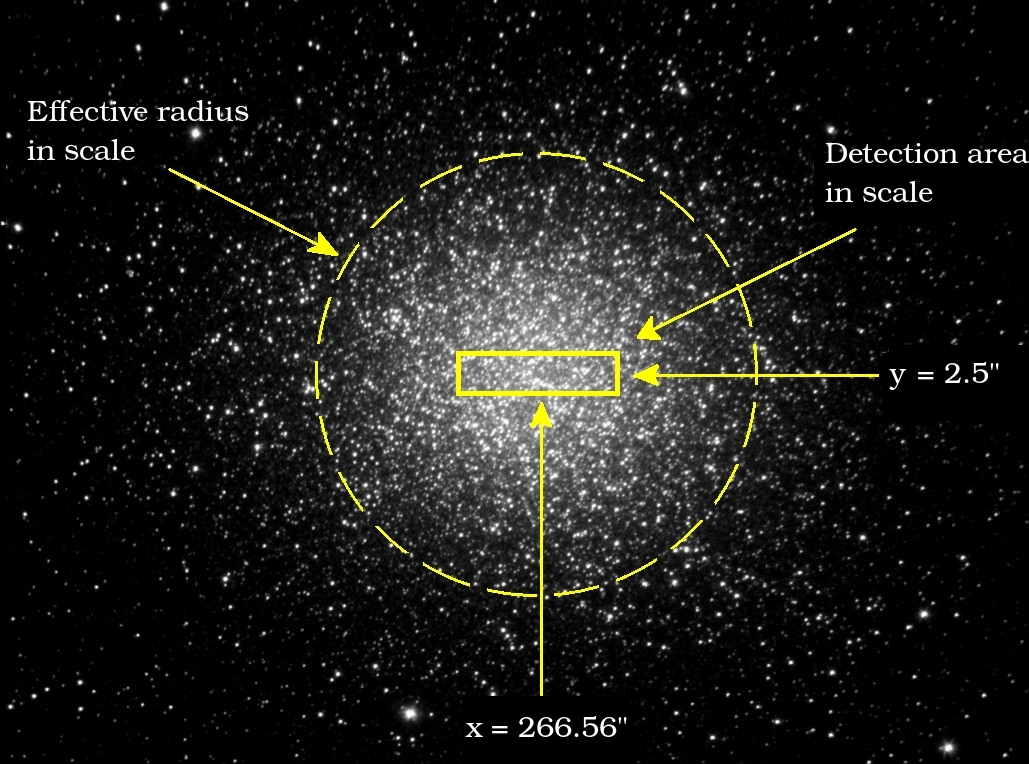
\includegraphics[width=12cm]{images/OmegaCentauriii.jpg}
\caption[Illustration of the detected area of the integrated spectrum]{Illustration of the detected area of the integrated spectrum of $\omega$ Centauri. The marked region represents the detected area in a bigger scale than it truly is, and has the angular dimensions shown in the figure. The dotted line represents the effective radius of the cluster (also in scale) that we use to extrapolate the results found for the detected area and make an approximation to what the whole stellar mass would be if we had an integrated spectrum of the whole globular cluster.}
\end{figure}

As this mass is the stellar mass contained only in the detection area (that in our set up configuration in OPD ends up to be $A_{D}=0.36\,pc^{2}$) we must extrapolate this result to its whole effective area to calculate the whole stellar mass of the system, noting that this will increase the error of the calculation.

If we take the cluster's tidal radius of 40' and it's distance to the Sun of $4,808.39\,pc$ using a distance modulus of 13.41, then the total effective area (where the stellar mass could be calculated using stellar population synthesis) is $A_{OC}=9,833.8\,pc^{2}$. 

Finally, the total stellar mass of the Cluster using this technique can be calculation using:

\begin{equation}
M_{s T} = N \times M_{\star}
\end{equation}

Where $N$ is the number of detection areas within the total effective area of Omega Centauri ($A_{OC}/A_{D}$) of about $31,844.8$. So that our calculation of the stellar mass is finally:

\begin{equation}
M_{s T} = 6.61 \times 10^{6}M_{\odot}
\end{equation}
 
This result is actually larger than some values  of the dynamical mass found in the literature and it should in principle, be smaller or at least equal to the dynamical mass, this discrepancy in our first approach to the mass determination is probably due to errors given by the extrapolation of the results of the detection area to the whole area of the cluster, because our detection area was very small compared to the cluster's size. Still, the stellar population technique is consistent with the order of magnitude of the cluster's mass previously reported. 

\subsection{Stellar scalength}

Because we wanted to be as accurate as possible in our modelling we found a way to calculate the stellar scalength and use it as a constraint to our modelling. We found the value of $a_{s}$ by fitting the effective radius in a de Vaucouleurs profile on the surface brightness of Eva Noyola's observational data of Omega Centauri (Noyola et al. 2013) shown in figure 4.6

\begin{figure}[H]
\centering
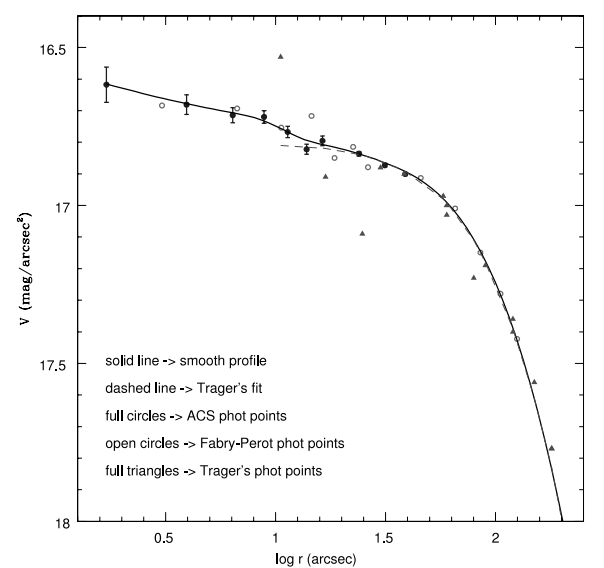
\includegraphics[width=8cm]{images/noyola.png}
\caption[Surface brightness profile of Omega Centauri]{Surface brightness profile for $\omega$ Centauri. The circles show Noyola's measured photometric points. The triangles show photometric points obtained from ground based images by Trager et al. The dashed line is Trager’s Chebychev fit. The solid line is Noyola's smooth fit that we don't use for our fitting of the scalength. Figure taken from Noyola et al. 2013}
\end{figure}

We fit the de Vaucouleurs profile (4.49) from Noyola's figure which is in terms of the surface brightness to this observational data 

\begin{equation}
\mu(r)=\mu_{e}+8.32678\left[\left(\frac{r}{R_{e}}\right)^{1/4}-1\right]
\end{equation}

The fitting gives an effective radius of $R_{e}=4.048pc$. We then use the relation $R_{e}\approx1.8153a$ (Hernquist 1989) that allows us to find a stellar scalength of our Hernquist profile of $a_{s}=2.23pc$. This is one of the constraints we use for some of our experiments.

\subsection{Central region}

Some authors (Jalali et al. 2012, Anderson \& Roeland. 2006) state that there might be a medium-mass black hole at the center of $\omega$ Centauri, so we need to take this into account if we want to make a proper modelling that is not affected by the presence of such a massive body in the velocity dispersion profile of the system.

In some of our experiments, we will include the central region of the cluster (0.5 to 2.0 arcmin) and in the other set of experiments we will exclude these regions. In terms of the estimated bins, it means that some of the experiments will use the two first radial bins and the other experiments won't. 

\section{Procedures}

For the mass modelling of the cluster, we do various experiments for studying its mass distribution using the solutions to equations 4.10, 4.13 and taking into account the mentioned constraints. In order to do so, we run 24 different experiments that consist on the variation of every parameter of our modelling (that is, dark matter mass $M_{dm}$, stellar mass $M_{s}$, dark matter scalength $a_{dm}$, stellar scalength $a_{s}$, mass-to-light ratio $\Gamma$ and parameter of anisotropy $\beta$) depending on the conditions that we set for each experiment individually. Our procedures follow this order:

First, we constraint half of our experiments to the total velocity dispersion profile including the center of the cluster (0.5 to 45 arcmin) and we call this set of experiments ``With Central Region"; the other half of the experiments is constrained to only the outer half of the cluster (2.0 to 45 arcmin) and we call them ``Without Central Region". Next, we use the constraints given by the mass to light ratio found in the literature in a series of experiments that we call ``Fixed $\Gamma$". Also we use the constraint of the stellar mass (found with Starlight) $M_s$ that we call ``Fixed $M_s$" and finally a set of experiments that don't have any of this constraints that we call ``Full".

Now, for each of this sets of experiments we apply some other constraints that are shown as follows: 

\textbf{\textit{i)}} In this one, we don't use the crossed terms ($\mathbf{B}(r)$ and $\mathbf{C}(r)$) in equation 4.13, because we wanted to see how relevant they were in the modelling, we call this ``\textbf{\textit{No crossed terms}}". 

\textbf{\textit{ii)}} We assume a constant stellar scalength, we call this ``\textbf{\textit{Fixed $a_{s}$}}", and we use the value of $2,23$ pc found with the surface brightness technique. 

\textbf{\textit{iii)}} We don't assume any of our parameters to be constant, that is, we vary $a_{s}$, $a_{dm}$, $\Gamma$, $\beta$, $M_{dm}$ and $M_{s}$ in the parameter matrix, we call this ``\textbf{\textit{Full}}". 

\textbf{\textit{iv)}} We assume the cluster doesn't have any dark matter so the solution of the equation 4.9 is much simpler and it's given by 4.10, we call this ``\textbf{\textit{No Dark matter}}".

Table 4.1 summarizes the experiments that we do and the order in which they were respectively done.

\begin{table}[H]
\centering
\label{my-label}
\begin{tabular}{|c|c|c|c|c|c|c|c|c|}
\hline
\multicolumn{1}{|c|}{\multirow{3}{*}{\textbf{Experiment}}} & \multicolumn{4}{c|}{\multirow{2}{*}{\textbf{With Central Region}}}                      & \multicolumn{4}{c|}{\multirow{2}{*}{\textbf{Without Central Region}}}                     \\
\multicolumn{1}{|l|}{}                  & \multicolumn{4}{c|}{}                                                                   & \multicolumn{4}{c|}{}                                                                    \\ \cline{2-9} 
\multicolumn{1}{|l|}{}                  & \textbf{Full}    & \textbf{Fixed $\Gamma$}    & \multicolumn{2}{c|}{\textbf{Fixed $M_s$}} & \textbf{Full}     & \textbf{Fixed $\Gamma$}     & \multicolumn{2}{c|}{\textbf{Fixed $M_s$}} \\ \hline
\textbf{No Crossed Terms}               & 1                & 5                       & $\sim$               & $\sim$              & 9                 & 13                       & $\sim$               & $\sim$              \\ \hline
\textbf{Fixed $a_s$}                       & 2                & 6                       & 17                   & 21                  & 10                & 14                       & 19                   & 23                  \\ \hline
\textbf{Full}                           & 3                & 7                       & 18                   & 22                  & 11                & 15                       & 20                   & 24                  \\ \hline
\textbf{No Dark Matter}                 & 4                & 8                       & $\sim$               & $\sim$              & 12                & 16                       & $\sim$               & $\sim$              \\ \hline
\end{tabular}
\caption[Characteristics of all the experiments]{Characteristics of all the experiments in our modelling. Every experiment is represented with a number for reference in the analysis section. For all the studied constraints (such as the central region, stellar mass, stellar scalength, etc), the experiments are organized as shown above.}
\end{table}

The method that we use for finding the best values of each and every parameter in our experiments had to be able to calculate several large integrals and optimize all the given parameters. For this purpose we wrote a set of C-based programs that contained the integrals given in equations 4.10 and 4.13 and used many \textit{gsl} routines that allow us to make integrals, interpolations of the analytic function and optimize the large number of calculations. Because the functions that we wanted to fit did not have an analytic solution, we decided use a $\chi^{2}$-like minimization method instead. 

This approximation method allows to fit curves to the observational data so that the parameters would be optimized, that is, the combination of parameters would allow the curve to fit well the observational data. Our programs were set so that the $\chi^{2}$ was calculated for every combination of the parameters (every entry of the parameters matrix) but it will only save the values of the parameters that make the smallest $\chi^{2}$. If we call $\sigma_{M}(r_{i})$ the value of our modelling for the radial bin $i$ and if $\sigma_{i}$ is the observational value of the projected velocity dispersion in the same bin, we show that our calculation of this approximation method is given by 

\begin{equation}
\chi^{2}=\sum_{i=1}^{n}\frac{1}{N_{i}}{\left(\sigma_{M}\left(r_{i}\right)-\sigma_{i}\right)}^{2}
\end{equation}

Where $N_{i}$ is the number of velocities used to calculate the velocity dispersion in bin $i$ (this was included to give more weight to the radial bins that were calculated with a higher number of data), and $n$ is the number of radial bins.

Because we needed to vary the parameters as much as possible to take into account all the entries of the parameter matrix. We started every experiment by running the programs with a large range using the literature data and reported values as a reference, and we used a big $\Delta$ for every parameter because the computational time required for every fit is too long for a small shift in the values of the parameters. This is summarized in table 4.2.

\begin{table}[H]
\centering
\label{my-label}
\begin{tabular}{|c|c|c|c|c|c|c|}
\hline
\multicolumn{7}{|c|}{\textbf{Thick Runs}}                                                                          \\ \hline
               & \textbf{$\mathbf{\Gamma}$} & \textbf{$\mathbf{\beta}$} & \textbf{$\mathbf{M_{s}}(10^{5} M_{\odot})$} & \textbf{$\mathbf{M_{dm}}(10^{5} M_{\odot})$} & \textbf{$\mathbf{a_{s}}(pc)$} & \textbf{$\mathbf{a_{dm}}(pc)$} \\ \hline
\textbf{$\mathbf{\Delta}$}  & 0.2  & 0.2      & 5.0     & 5.0     & 5.0      & 5.0            \\ \hline
\textbf{Range} & 0.1 - 3.0      & 0.001 - 1.0        & 1.0 - 80.0      & 1.0 - 80.0   & 1.0 - 60.0      & 1.0 - 60.0            \\ \hline
\end{tabular}
\caption[Thick runs characteristics]{Characteristics of the first runs of our modelling that involve a huge range in the parameter space (to reach for all the possible values of the parameters) and a thick $\Delta$ (for computational time purposes).}
\end{table}

After these programs have been run, and we have found some values of the parameters that best fit the observational data, we do a second run of the programs for each experiments with a smaller $\Delta$ around the fitted parameter in the first run to make a better approximation of the real values as shown in table 4.3.

\begin{table}[H]
\centering
\label{my-label}
\begin{tabular}{|c|c|c|c|c|c|c|}
\hline
\multicolumn{7}{|c|}{\textbf{Refined Runs}}                                                                          \\ \hline
               & \textbf{$\mathbf{\Gamma}$} & \textbf{$\mathbf{\beta}$} & \textbf{$\mathbf{M_{s}}(10^{5} M_{\odot})$} & \textbf{$\mathbf{M_{dm}}(10^{5} M_{\odot})$} & \textbf{$\mathbf{a_{s}}(pc)$} & \textbf{$\mathbf{a_{dm}}(pc)$} \\ \hline
\textbf{$\mathbf{\Delta}$}  &  0.1 &  0.01     &  0.2    &  0.2   &  0.2    &  0.2          \\ \hline
\textbf{Range} & $\Gamma_{1}\pm 0.2$   & $\beta_{1}\pm 0.03$        & $M_{s}_{1}\pm 2.0$      & $M_{dm}_{1}\pm 2.0$   & $a_{s}_{1}\pm 2.0$      & $a_{dm}_{1}\pm 2.0$            \\ \hline
\end{tabular}
\caption[Characteristics of the refined runs of the modelling]{Characteristics of the refined runs of the modelling. Note that the range used in these runs is a small region around the values found with the thick runs of the programs. Also, the $\Delta$ around which the parameters change is very small compared to the thick runs, so that the fitting of all the parameters is effectively refined.}
\end{table}

We noticed that this two-step approach produces results that can give us a degree of precision that is enough for us to trust so we didn't need a more sophisticated parameter exploration technique. In fact, the size of the grids of the refined runs of the models is 4\% the size of the grid in the thick runs, meaning that the degree of precision is much larger. In the case of the scalengths for example, this precision happens to be be of the order of tenths of parsecs that can be a good for a first approach to the modelling of the cluster.

The results and interpretation of all the experiments are explained in the next section.

\section{Results}

In this section, we discuss the results given by the fitting of all the conducted experiments after the refined runs of the programs have been made. Every experiment will be referred to its given number in table 4.1, where its characteristics are explicitly shown.

\subsection{Full fits with inner region (Experiments 1, 2, 3 and 4)}

This set of experiments consist on the variation of all the parameters with the velocity dispersion profile that includes the central region of the globular cluster (0.5 to 2.0 arcmin or the first two radial bins in figure 4.1). The results of the fitted curve with the optimized parameters are shown in figure 4.7

\begin{figure}[]
\centering
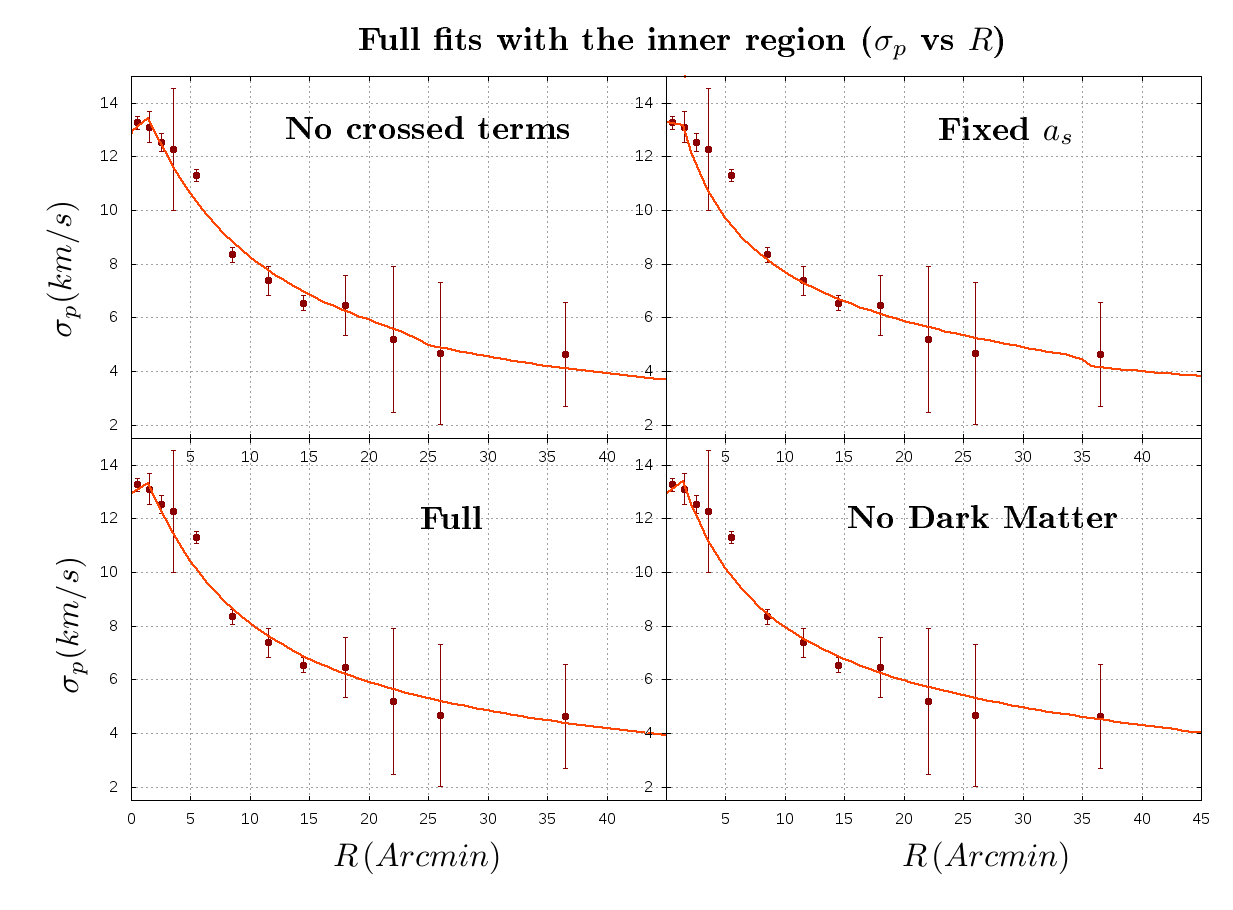
\includegraphics[width=15cm]{images/all_params_refinado_12.png}
\caption[Best fit of the full model with the inner region]{Best fit to the observational data of experiments 1,2,3, and 4 for our full model with the inner region of the cluster (in orange) and the observational data of radial velocity dispersions in the chosen radial bins (red). They are shown in different plots because in some cases they overlap too much for their behaviour to be clearly seen.}

\end{figure}

Note that in figure 4.7, the fitted curves reproduced the observational data consistently although every line has its own characteristics. In the case of experiments 1,3 and 4, there is an awkward behaviour of the line in the inner region that didn't seem to be a problem in the solution of the large integrals in equation 4.13 so it could be due to physical reasons such as a massive body in that region as suggested by Jalali et al. 2012 (we need to make a proper modelling of the centre of the cluster including the term of the potential produced by such as massive body). In the second experiment, there can be seen another unusual feature of the curve around 37 arcmin that is due to the way that the integrals $\mathbf{A}(r)$, $\mathbf{B}(r)$, $\mathbf{C}(r)$ and $\mathbf{D}(r)$ contribute to equation 4.13 because $\sigma_{p}$ is a sum of those integrals. Although this strange feature is present in many of the experiments, we must mention that it does not change significantly the results of the fitting of the curve to the observational data. 

The fitted values for the parameters that reproduce figure 4.7 are shown in table 4.4.

\begin{table}[H]
\centering
\begin{tabular}{| c | c | c | c | c | c | c| }
    \hline
    \textbf{Experiment} & $\mathbf{\beta}$ & $\mathbf{a_{dm}} (pc)$ & $\mathbf{a_{s}} (pc)$ & $\mathbf{M_{dm}}$ ($M_{\odot}$) & $\mathbf{M_{s}}$ ($M_{\odot}$) & $\mathbf{\Gamma}$\\ \hline
	No Crossed terms (1) & $0.62$ &	$15.8$ &	$29.0$ &	$5.6 \times 10^{5}$ &	$8.0 \times 10^{4}$ &	$2.2$\\ \hline
	Fixed $a_s$ (2) &	$0.0001$ &	$9.0$ &	$\mathbf{2.23}$ &	$1.12 \times 10^{5}$ &	$1.06 \times 10 ^{6}$ &	$1.5$\\ \hline
	Full (3) &	$0.46$ &	$15.2$ &	$52.6$ &	$9 \times 10^{5}$ &	$9 \times 10^{5}$ &	$0.38$\\ \hline
	No Dark Matter (4) &	$0.26$ & $\thicksim$	& $3.64$  & $\thicksim$ & $  1.98 \times 10^{6}$ & 	$1.24$\\
    \hline
  \end{tabular} 
\caption[Optimized parameters for our full model with the inner region.]{The optimized parameters for each of the experiments for our full model with the inner region of the cluster. Note that there are not any values in the $4 ^{th}$ experiment for the dark matter scalength and mass because this model assumes that the only contributions are given by the stars of the system and there is not a dark matter component. The fixed stellar scalength found with photometry procedures is put in bold cases because it is one of our most important and reliable constraints.}
\end{table}

We don't note any special trend in the anisotropy parameter because it spans in pretty much all the range that was allowed, except for the second experiment where it has the smallest possible value. We can also note a very small value for the mass-to-light ratio in the third experiment but it doesn't really give us any special information until we see any trend with the other experiments. In the case of the scalengths we note that the dark matter scalength is bigger than the stellar scalength in experiment 2 where we set $a_s$ as a fixed parameter, but in the other cases $a_{dm}<a_s$ which suggests a more concentrated dark matter distribution. The constraint of the stellar scalength is one of our most reliable constraints because it was estimated using strong physical reasons and very accurate procedures so we expect the stellar scalengths of the other fits to be close to this value ($2.23$ pc). 

It's important to note that the results of experiment 4 are very close to the reported values in the literature and reproduce quite well the stellar scalength that we found using photometry. This might suggest that the model with no dark matter is the right model, but as we shall discuss in the conclusions, this statement has to be treated carefully given all the results of the experiments. As a very important conclusion about these results we may note that the results of experiments 2 and 4 are comparable and reproduce quite well the literature data not only in the scalengths but also in the total mass associated to them.

The following group of experiments don't take into account the inner region of the cluster.

\subsection{Full fits without the inner region (Experiments 9, 10, 11 and 12)}

In this set of experiments we use only the outer region of the cluster (2.0 to 45 arcmin) because we want to avoid the problems in the center and search for a smoother behaviour in the fitting of our model. 

Figure 4.8 shows the fitted lines for experiments 9, 10, 11 and 12. The first thing we notice is that the strange behaviour in the centre of the cluster is different than in the previous fits, and is only shown in experiments 9 and 11. The curves are satisfactory because they fit very well the observational data and show a smooth behaviour as expected. The strange feature in the ``Fixed $a_s$" experiment (2) in the previous experiments is not observed in (10).

\begin{figure}[H]
\centering
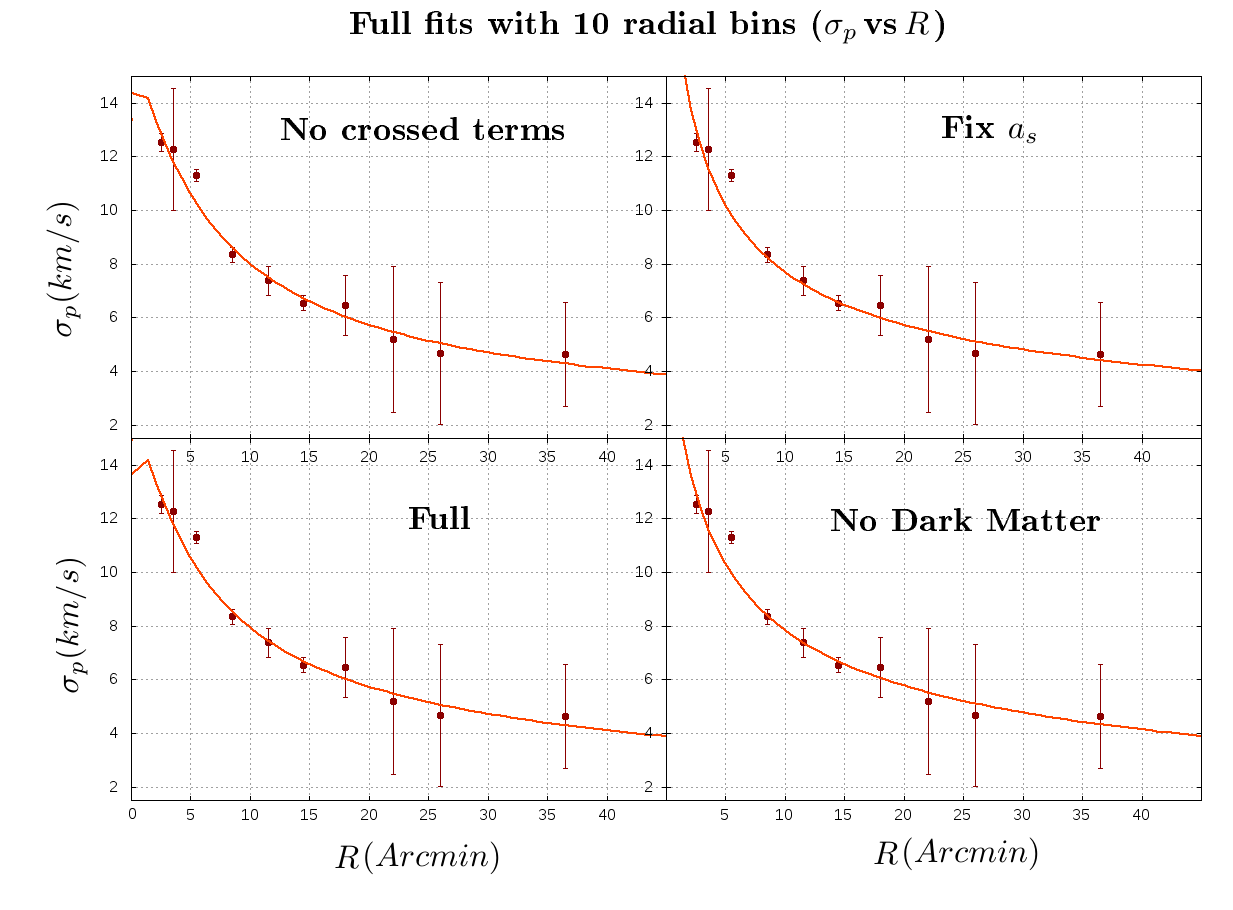
\includegraphics[width=15cm]{images/all_params_refinado_10.png}
\caption[Best fit of the full model without the inner region]{Best fit to the observational data of the four experiments for our full model without the inner region of the cluster.}
\end{figure}

The optimized parameters for this set of experiments are displayed in table 4.5.

\begin{table}[H]
\centering
\begin{tabular}{| c| c| c| c| c| c| c|}
    \hline
    \textbf{Experiment} & $\mathbf{\beta}$ & $\mathbf{a_{dm}} (pc)$ & $\mathbf{a_{s}} (pc)$ & $\mathbf{M_{dm}}$ ($M_{\odot}$) & $\mathbf{M_{s}}$ ($M_{\odot}$) & $\mathbf{\Gamma}$\\ \hline
	No Crossed terms (9) & $0.6$ &	$16$ &	$52.8$ &	$2.1 \times 10^{6}$ &	$2.72 \times 10^{6}$ &	$2.3$\\ \hline
	Fixed (10) $a_s$ &	$0.79$ &	$57.9$ &	$\mathbf{2.23}$ &	$8 \times 10^{5}$ &	$3.43 \times 10 ^{6}$ &	$2.1$\\ \hline
	Full (11) &	$0.04$ &	$11.8$ &	$57.8$ &	$6 \times 10^{5}$ &	$9 \times 10^{5}$ &	$2.1$\\ \hline
	No Dark Matter (12) &	$0.78$ &	$\thicksim$ & $2.96$ &	$\thicksim$ & $ 3 \times 10^{6}$ & 	$1.94$\\
    \hline
  \end{tabular} 
\caption[Optimized parameters for our full model without the inner region.]{The optimized parameters for each of the experiments for our full model without the inner region of the cluster.}
\end{table}

There's a clear trend in the mass values as seen in table 4.5, the stellar mass is bigger than the dark matter mass in experiments 9, 10 and 11 and the total mass of the four experiments reproduce the same order of magnitude reported in the literature, these results suggest that the dark matter mass in the stellar system is just a small fraction of the total mass but only if the other physical parameter (stellar scalength) is consistent with the expected value. 

As is can be seen in experiments 9 and 11, the stellar scalength is way too large compared to the one estimated with Noyola's photometric data so these results are not very consistent and don't allow us to give a good degree of confidence to the masses found with these experiments. 

On the other hand, the values found in experiment 10 and 12 are comparable, and very consistent with the values found in the literature for the stellar scalength and the total dynamical mass. In experiment 10 the dark matter scalength is very large compared to $a_s$ and the dark matter mass is smaller than the one associated to stars so we may think that the dark matter halo of the system is more diluted and less massive. The model that doesn't involve dark matter (12) is also consistent with the results of experiment 10 showing the same trend seen in experiments 2 and 4.  

\subsection{Fixed $\Gamma$ with the inner region (Experiments 5, 6, 7 and 8)}

In the following set of experiments, we constrained the mass-to-light ratio to that found by Van de Ven et al. 2005 with a value of $\Gamma = 2.5$. 

The first group of experiments are 5, 6, 7 and 8 as named in table 4.1. The constant mass-to-light ratio $\Gamma$ allows us to use a smaller grid for the parameters even in the thick runs because the number of iterations is reduced when we fix one of the parameters in the programs. The fitted curves are shown in figure 4.9. 

\begin{figure}[H]
\centering
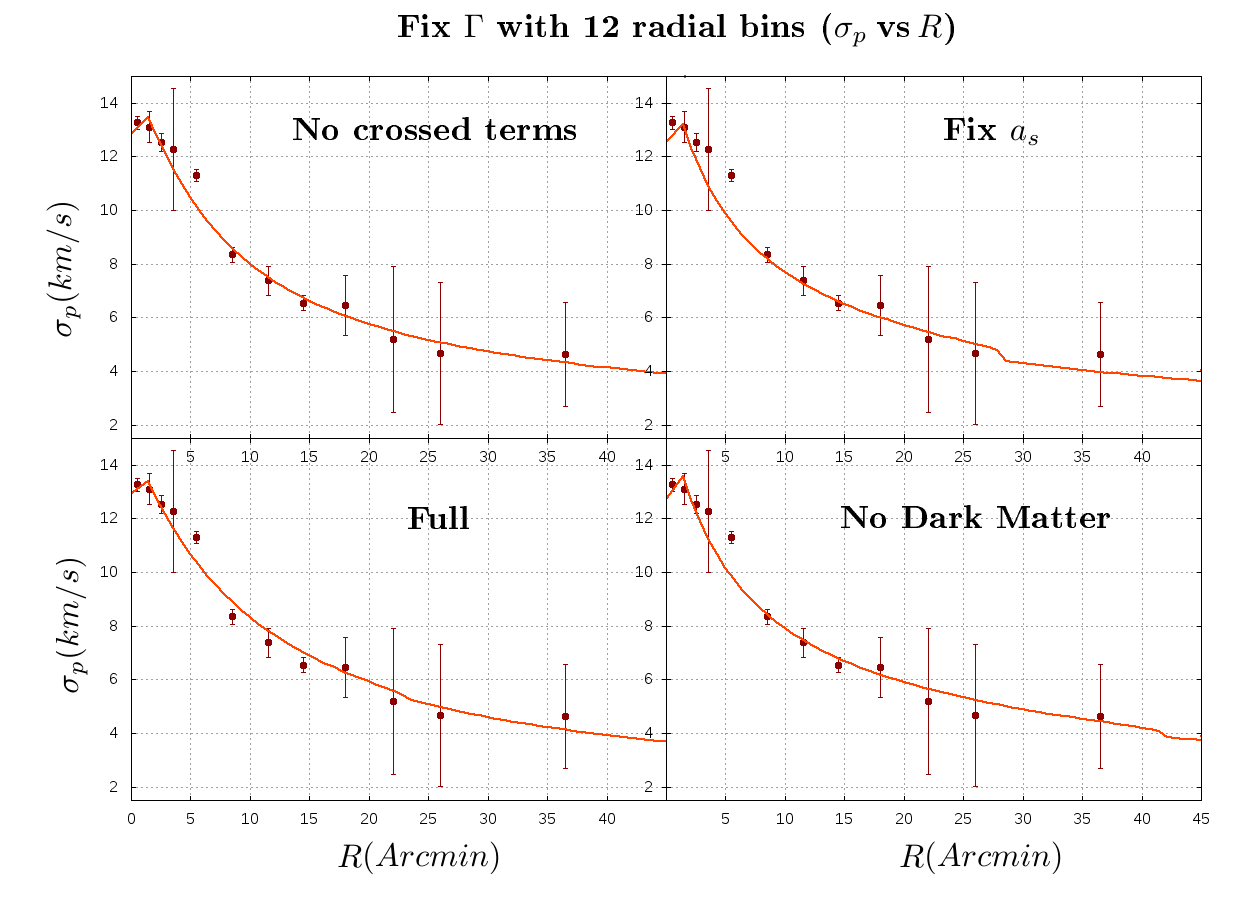
\includegraphics[width=15cm]{images/fix_gamma_refinado_12.png}
\caption[Best fit of our model with a fix mass-to-light ratio with the inner region]{Best fit to the observational data of the four experiments for our model with a fix mass-to-light ratio with the inner region of the cluster.}
\end{figure}

The first thing we note in figure 4.9 is the presence of the strange feature in the innermost region of the cluster in the four experiment that need to be addressed with a more precise modelling of the centre of the cluster. Although the curves adjust well to the velocity dispersion profile, experiments 6 and 8 show another strange feature (again due to the way that the integrals $\mathbf{A}(r)$, $\mathbf{B}(r)$, $\mathbf{C}(r)$ and $\mathbf{D}(r)$ contribute to equation 4.13) towards the end of the curve that doesn't affect strongly the fitting but needs to be taken into consideration.

Table 4.6 shows the optimized values of the parameters of the curves shown in figure 4.9.

\begin{table}[H]
\centering
%\begin{center}
\begin{tabular}{| c| c| c| c| c| c| c|}
    \hline
    \textbf{Experiment} & $\mathbf{\beta}$ & $\mathbf{a_{dm}} (pc)$ & $\mathbf{a_{s}} (pc)$ & $\mathbf{M_{dm}}$ ($M_{\odot}$) & $\mathbf{M_{s}}$ ($M_{\odot}$) & $\mathbf{\Gamma}$\\ \hline
	No Crossed terms (5) & $0.35$ &	$16.4$ &	$55.62$ &	$1.62 \times 10^{6}$ &	$2.1 \times 10^{6}$ &	$2.5$\\ \hline
	Fixed $a_s$ (6) &	$0.001$ &	$3.0$ &	$\mathbf{2.23}$ &	$3 \times 10^{5}$ &	$5.0 \times 10 ^{5}$ &	$2.5$\\ \hline
	Full (7) &	$0.72$ &	$20.0$ &	$44.4$ &	$5.2 \times 10^{5}$ &	$8.0 \times 10^{4}$ &	$2.5$\\ \hline
	No Dark Matter (8) &	$0.001$ &	$\thicksim$ & $ 3.15$ &	$\thicksim$ & $ 1.52 \times 10^{6}$ & 	$2.5$\\
    \hline
  \end{tabular} 
\caption[Optimized parameters for our fix mass-to-light ratio model with the inner region.]{The optimized parameters for each of the experiments for our fix mass-to-light ratio model with the inner region of the cluster.}
%\end{center}
\end{table}

The trends of experiments 5, 6, 7 and 8 don't differ too much from the ones of experiments 1, 2, 3 and 4 although the values are quite different, it is worth noting that the experiment with no dark matter still reproduces quite well the literature data. The ``Fixed $a_s$" experiment gives a small total mass where the mass associated to dark mater is again smaller than the one associated to the stars of the system. In all the experiments so far, we have seen that the ones where the crossed terms are not taken into account deviate too much from the other experiments so that we may not trust these results. 

The stellar scalengths for experiments 5 and 7 are again too large compared to the one found with Noyola's data. As these results don't match one of our most trustworthy constraints, we don't focus our conclusions on their results but we take them into account to understand a very important fact in our modelling regarding the fundamental relationship between the stellar scalengths and the masses found with the models. The masses found in the models are linked directly to the value of $a_s$ because the functional form of equation 4.13 links those parameters explicitly in the crossed terms $\mathbf{B}(r)$, $\mathbf{C}(r)$ and in the surface brightness $I(R)$. It would be impossible for example to switch $a_s$ of $a_{dm}$ in that equation if we want to fit the correct values for $M_s$ and $M_{dm}$. 

The relationship between the masses and the scalengths is very important because it allows us to see how consistent a model is by seeing how these parameters are correlated and put in terms of all the other constraints. For example, in experiment 7, the stellar scalength is very large compared to the trusted value of $2.23$ and the total dynamical mass ($M_{s}+M_{dm}$) is too small compared to the literature data, so we see that a value of $a_s$ that deviates too much from the literature value yields masses that are not very consistent as well.  

\subsection{Fixed $\Gamma$ without the inner region (Experiments 13, 14, 15 and 16)}

Again, we set the mass-to-light ratio to $2.5$ and vary the rest of the parameters excluding the inner region of the cluster (0.5-2.0 arcmin) in experiments 13, 14, 15 and 16. The fitted curves are shown in figure 4.10

\begin{figure}[H]
\centering
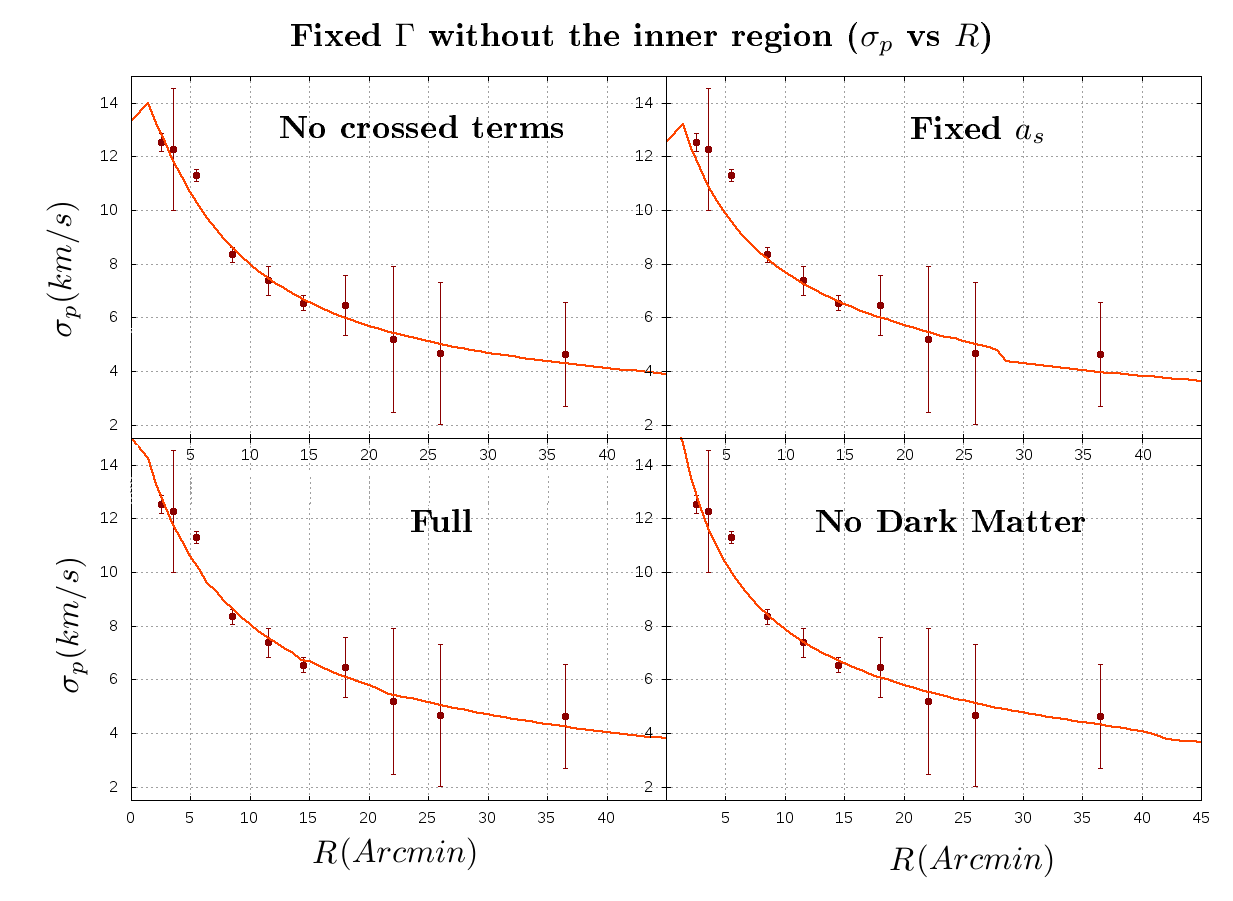
\includegraphics[width=15cm]{images/fix_gamma_refinado_10.png}
\caption[Best fit of our model with a fix mass-to-light ratio without the inner region]{Best fit to the observational data of the four experiments for our model with a fix mass-to-light ratio without the inner region of the cluster.}
\end{figure}

We note that the strange features in the innermost region are clearly visible in experiments 13 and 14, and also an unusual behaviour of the curve around 27 arcmin in experiment 14. The optimized parameters are shown in table 4.7.

\begin{table}[H]
\centering
\begin{tabular}{| c| c| c| c| c| c| c|}
    \hline
    \textbf{Experiment} & $\mathbf{\beta}$ & $\mathbf{a_{dm}} (pc)$ & $\mathbf{a_{s}} (pc)$ & $\mathbf{M_{dm}}$ ($M_{\odot}$) & $\mathbf{M_{s}}$ ($M_{\odot}$) & $\mathbf{\Gamma}$\\ \hline
	No Crossed terms (13) & $0.2$ &	$15.2$ &	$59.8$ &	$1.4 \times 10^{6}$ &	$2.1 \times 10^{6}$ &	$2.5$\\ \hline
	Fixed $a_s$ (14) &	$0.801$ &	$3.0$ &	$\mathbf{2.23}$ &	$5 \times 10^{5}$ &	$1.0 \times 10 ^{5}$ &	$2.5$\\ \hline
	Full (15) &	$0.9$ &	$16.0$ &	$44.6$ &	$1.62 \times 10^{6}$ &	$1.42 \times 10^{6}$ &	$2.5$\\ \hline
	No Dark Matter (16) &	$0.38$ &	$\thicksim$ & $ 2.38$ &	$\thicksim$ & $  2.03 \times 10^{6}$ & 	$2.5$\\
    \hline
  \end{tabular} 
\caption[Optimized parameters for our fix mass-to-light ratio model without the inner region.]{The optimized parameters for each of the experiments for our fix mass-to-light ratio model without the inner region of the cluster.}
\end{table} 

We see that although the total mass in experiments 13 and 15 are consistent with the literature, their stellar scalengths are too large to be very reliable results. Once again, the experiment with no dark matter reproduces quite well the dynamical mass of the cluster reported in the literature and its stellar scalength is very close to the value found with photometry. 

This time, the experiment with the fixed stellar scalength yields a total dynamical mass that is very small compared to the reported values in table 2.1 because it doesn't even reach the same order of magnitude. It is quite interesting that the two consistent experiments (the ones with ``Fixed $a_s$" and ``No Dark Matter") in these experiments in particular give a very small value for the parameter of anisotropy  due to the fixed mass-to-light ratio of 2.5. 

Excluding the innermost region of the globular cluster yields a much larger total mass for the experiments where $a_s$ is also a free parameter (Experiment 7 and 15). Now, we set the constraint of a stellar mass to the mass that we found with Starlight and get the following results.

\subsection{Fixed Stellar Mass with the inner region (Experiments 17 and 18)}

We noted that the experiments where we didn't use the crossed terms in equation 4.13 showed different results from the experiments where we solved the whole equation, plus, there is not any physical reason to exclude these terms in the equation. This means that those crossed terms need to be included in the correct fitting so we decided not to waste time running the ``No Crossed Terms" models in the next group of experiments. Also, the ``No Dark Matter" experiments are not conducted since we would already be constraining the total mass to be the stellar mass found with Starlight so that it would be a waste of time to run those programs.

The experiments we run are ``Full" and ``Fix $a_s$" named as 17 and 18 (in consonance with the previous results) in table 4.1 and the results are shown in figure 4.11.

\begin{figure}[H]
\centering
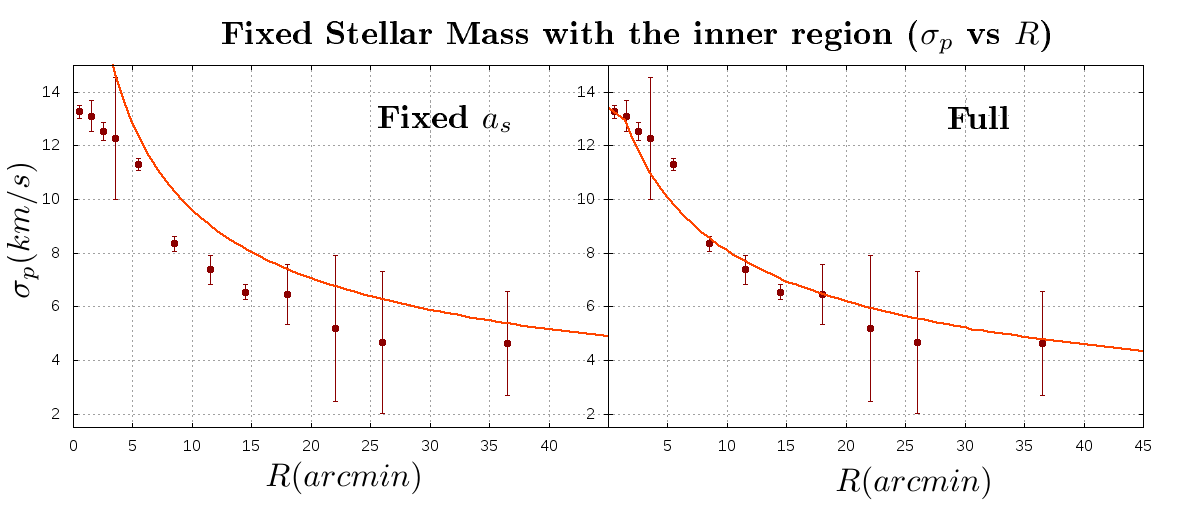
\includegraphics[width=15cm]{images/Starlight_2.png}
\caption[Best fit of our model with the mass found with the Starlight procedures with the inner region]{Best fit to the observational data of the four experiments for our model with the Starlight procedures with the inner region of the cluster.}
\end{figure}

Note that the fitting with a fixed stellar scalength (experiment 17) was very bad because it doesn't even pass through the observational points, so it didn't give us any valuable result for any of the parameters, but it allows us to question if setting a smaller value of $M_s$ would produce a better fitting and pass through the observational points (this experiment is done in experiments 21, 21, 23 and 24). The fitted parameters for both experiments are shown in table 4.8. 

\begin{table}[H]
\centering
\begin{tabular}{| c| c| c| c| c| c| c|}
    \hline
    \textbf{Experiment} & $\mathbf{\beta}$ & $\mathbf{a_{dm}} (pc)$ & $\mathbf{a_{s}} (pc)$ & $\mathbf{M_{dm}}$ ($M_{\odot}$) & $\mathbf{M_{s}}$ ($M_{\odot}$) & $\mathbf{\Gamma}$\\ \hline
	Fixed $a_s$ (17) &	$0.88$ &	$56.98$ &	$\mathbf{2.23}$ &	$8 \times 10^{4}$ &	$6.61 \times 10 ^{6}$ &	$1.6$\\ \hline
	Full (18) &	$0.96$ &	$7.6$ &	$12.0$ &	$6.88 \times 10^{5}$ &	$6.61 \times 10^{6}$ &	$0.9$\\ \hline
  \end{tabular} 
\caption[Optimized parameters for our model with the mass found with the Starlight procedures with the inner region.]{The optimized parameters for each of the experiments for our model with the mass found with the Starlight procedures with the inner region of the cluster.}
\end{table}

The first thing we notice is that the dark matter masses in both experiments are way smaller than the stellar mass found with Starlight (as it was expected because the Starlight procedures yielded a very large value for $M_s$) so the total mass can't be any larger for the modelling to be consistent. 

The dark matter scalength is very large in the experiment with the fixed $a_s$ and the mass is too small so this fitting evidently has a non-consistent result that is also shown in figure 4.11. 

The anisotropy parameter is very large and although not shown explicitly, the $\chi^{2}$ values are very large meaning that the fittings were not as good as in the previous experiments.

\subsection{Fixed Stellar Mass without the inner region (Experiments 19 and 20)}

Once again, we want to see how the centre of the cluster affects our results so we run experiments 19 and 20 for the outer region of $\omega$ Centauri. The fitted curves are shown in figure 4.12. 

\begin{figure}[H]
\centering
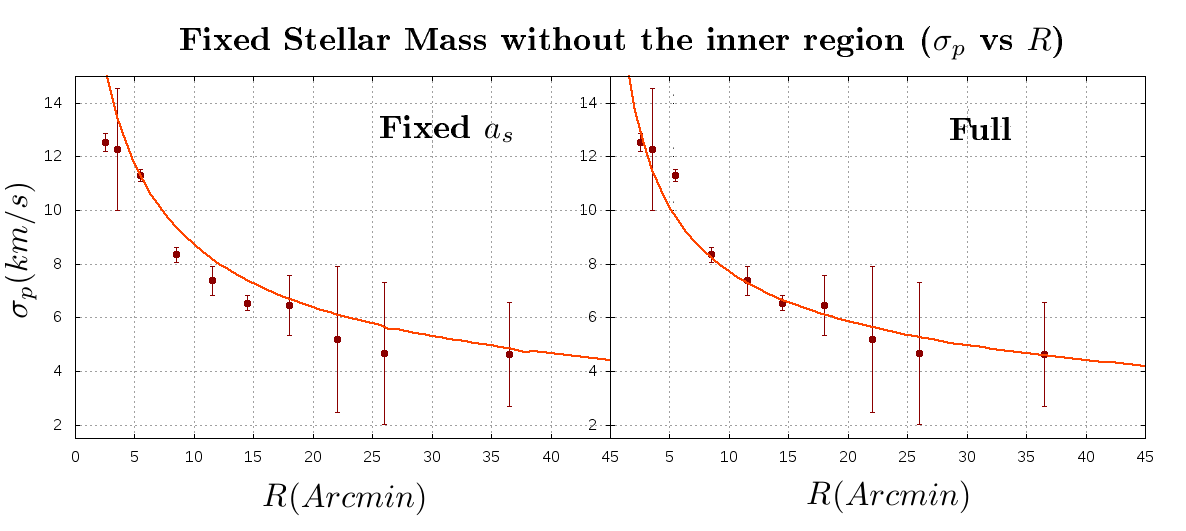
\includegraphics[width=15cm]{images/Starlight_1.png}
\caption[Best fit of our model with the mass found with the Starlight procedures without the inner region]{Best fit to the observational data of the four experiments for our model without the Starlight procedures with the inner region of the cluster.}
\end{figure}

The curves reproduce better the observational data than in the previous fit, but still the $\chi^{2}$ value is not too satisfactory. This can be understood since the stellar mass is too large and the dark matter mass has to be very small to reach a small minimization value. The fit parameter values are shown in table 4.9.

\begin{table}[H]
\centering
\begin{tabular}{| c| c| c| c| c| c| c|}
    \hline
    \textbf{Experiment} & $\mathbf{\beta}$ & $\mathbf{a_{dm}} (pc)$ & $\mathbf{a_{s}} (pc)$ & $\mathbf{M_{dm}}$ ($M_{\odot}$) & $\mathbf{M_{s}}$ ($M_{\odot}$) & $\mathbf{\Gamma}$\\ \hline
	Fixed $a_s$ (19) &	$0.95$ &	$58.0$ &	$\mathbf{2.23}$ &	$8 \times 10^{4}$ &	$6.61 \times 10 ^{6}$ &	$2.3$\\ \hline
	Full (20) &	$0.96$ &	$7.36$ &	$50.0$ &	$1.35 \times 10^{6}$ &	$6.61 \times 10^{6}$ &	$1.88$\\ \hline
  \end{tabular} 
\caption[Optimized parameters for our model with the mass found with the Starlight procedures without the inner region.]{The optimized parameters for each of the experiments for our model with the mass found with the Starlight procedures without the inner region of the cluster.}
\end{table}

The results of these experiments are very similar to those of experiments 17 and 18 because $M_{s}>M_{dm}$ by a big factor and the scalengths are too different showing no consistency with the expected values that should in principle be comparable values. The anisotropy parameter is again very large in contradiction to what we may expect taking the literature values as a reference.

As it can be seen most of the experiments that we have discussed, there is an interesting trend in the results that suggest that there is in fact a dark matter contribution but it is smaller than the baryonic matter and it is more diluted (a bigger scalength is associated to dark matter) so for the final set of experiments we decided to set a fixed value for the stellar mass that is in concordance with the literature so that we can see if this statement is consistent with the results of these experiments. 

The value that we are going to use for the stellar mass is $M_{s}=2.0 \times 10^{6} M_{\odot}$

\subsection{Final Fixed Stellar Mass with the inner region (Experiments 21 and 22)}

For experiments 21 and 22 consider the innermost region of the cluster and the fitted curves are shown in figure 4.13

\begin{figure}[H]
\centering
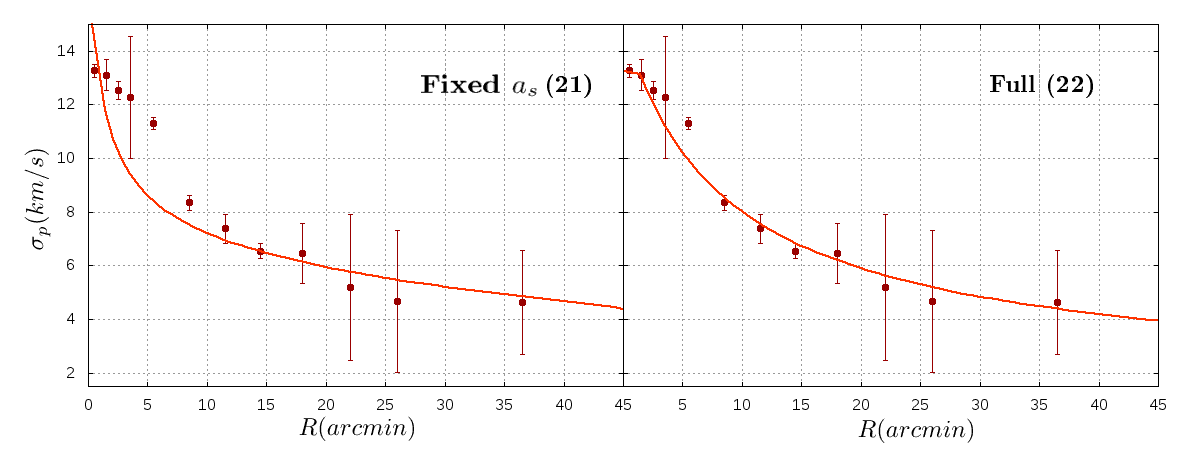
\includegraphics[width=15cm]{images/Starlight_25_12_1.png}
\caption[Best fits for our model with a mass value based on the Starlight procedures with the inner region.]{Best fit for each of the experiments for our model with a mass value of $2.0 \times 10^{6} M_{\odot}$ with the inner region of the cluster.}
\end{figure}

We note that the form of the curve in experiment 21 is very different from experiments 17 and 19 but the value found for the $\chi^{2}$ is a bit smaller and it made the curve go down vertically so that it crossed the observational data, just like we guessed when we used a smaller value for the stellar mass. A consistent value used for $M_s$ allows for a better optimization of the parameters and we find that these values are in fact more consistent with the literature data. Table 4.10 shows these values.

\begin{table}[H]
\centering
\begin{tabular}{| c| c| c| c| c| c| c|}
    \hline
    \textbf{Experiment} & $\mathbf{\beta}$ & $\mathbf{a_{dm}} (pc)$ & $\mathbf{a_{s}} (pc)$ & $\mathbf{M_{dm}}$ ($M_{\odot}$) & $\mathbf{M_{s}}$ ($M_{\odot}$) & $\mathbf{\Gamma}$\\ \hline
	Fixed $a_s$ (21) &	$0.86$ &	$15.0$ &	$\mathbf{2.23}$ &	$5.88 \times 10^{5}$ &	$2.0 \times 10 ^{6}$ &	$0.3$\\ \hline
	Full (22) &	$0.96$ &	$19.8$ &	$50.0$ &	$2.1 \times 10^{6}$ &	$2.0 \times 10^{6}$ &	$1.36$\\ \hline
  \end{tabular} 
\caption[Optimized parameters for our model with a mass value based on the Starlight procedures with the inner region.]{The optimized parameters for each of the experiments for our model with a mass value of $2.0 \times 10^{6} M_{\odot}$ with the inner region of the cluster.}
\end{table}

The experiment with the fixed stellar scalength $a_s$ (experiment 21) gives a very small value for the dark matter mass as oppose to experiment 22 where $M_{dm}$ is of the same order of magnitude. In experiment 21, $a_{dm}$ is very large compared to $a_s$ which suggests (like in previous results) that if there is a dark matter halo in the stellar system, then it would be more diluted than the halo of the stellar mass. Experiment 22 yielded a stellar scalength too large to be consistent with our trusted value of $2.23$ and the total mass in the experiment is also very large compared to the values in table 2.1. 

Most importantly, this experiment confirms our previous suggestion that said that setting a smaller $M_s$ would give more consistent results on the fitted parameters.

\subsection{Final Fixed Stellar Mass without the inner region (Experiments 23 and 24)}

And finally, excluding the innermost region of the cluster, we have the results of the best fits shown in figure 4.14

\begin{figure}[H]
\centering
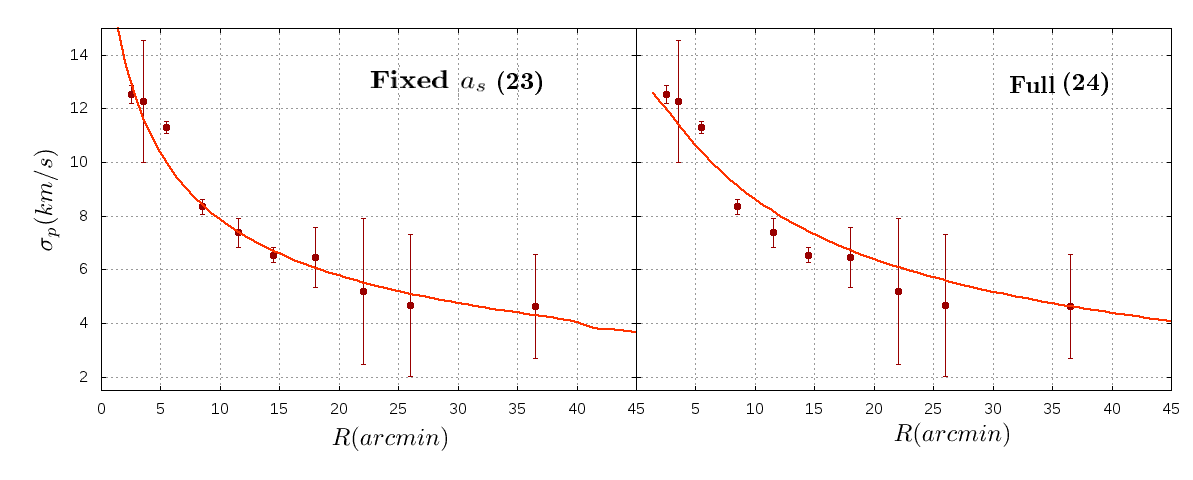
\includegraphics[width=15cm]{images/Starlight_25_10_1.png}
\caption[Best fits for our model with a mass value based on the Starlight procedures without the inner region.]{Best fit for each of the experiments for our model with a mass value of $2.0 \times 10^{6} M_{\odot}$ without the inner region of the cluster.}
\end{figure}

Again, the use of a consistent $M_s$ allows for a good fitting of the curve as it can be seen in figure 4.14. The $\chi^{2}$ value for both experiments was also small compared to the one in experiments 19 and 20. The fitted parameter values are shown in table 4.11

\begin{table}[H]
\centering
\begin{tabular}{| c| c| c| c| c| c| c|}
    \hline
    \textbf{Experiment} & $\mathbf{\beta}$ & $\mathbf{a_{dm}} (pc)$ & $\mathbf{a_{s}} (pc)$ & $\mathbf{M_{dm}}$ ($M_{\odot}$) & $\mathbf{M_{s}}$ ($M_{\odot}$) & $\mathbf{\Gamma}$\\ \hline
	Fixed $a_s$ (23) &	$0.5$ &	$3.1$ &	$\mathbf{2.23}$ &	$1.36 \times 10^{6}$ &	$2.0 \times 10 ^{6}$ &	$0.64$\\ \hline
	Full (24) &	$0.48$ &	$19.98$ &	$53.0$ &	$1.8 \times 10^{6}$ &	$2.0 \times 10^{6}$ &	$2.1$\\ \hline
  \end{tabular} 
\caption[Optimized parameters for our model with a mass value based on the Starlight procedures without the inner region.]{The optimized parameters for each of the experiments for our model with a mass value of $2.0 \times 10^{6} M_{\odot}$ without the inner region of the cluster.} 
\end{table}

In both cases (experiments 23 and 24), the dark matter mass is just a little bit smaller than the mass associated to the stars, but is very close to it and in the same order of magnitude, but the stellar scalength in experiment 24 is way too large to be comparable to the one in experiment 23 that (as we have seen in all the previous experiments) seems to be the best modelling with the very interesting results that suggest that the cluster has a diluted dark matter halo that is less massive than the one associated to the stars in the system.

 The final conclusions of all of the conducted experiments and the modelling as a whole are discussed in the following chapter.